\documentclass[conference]{IEEEtran}
\usepackage[utf8]{inputenc} 
\usepackage[T1]{fontenc} 
\usepackage[croatian]{babel}
\usepackage{url}
\usepackage{amsfonts}
\hyphenation{op-tical net-works semi-conduc-tor}
\usepackage{amsmath}
\usepackage{graphicx}
\usepackage{multirow}
\usepackage[table,xcdraw]{xcolor}
\graphicspath{ {/home/gorana/projects/machine_learning/projekt/strojno-ucenje/data/cross-validation/} }
\begin{document}
\title{Ekstrakcija likova iz kratkih priča}
\author{\IEEEauthorblockN{Gorana Levačić}
\and
\IEEEauthorblockN{Tomislav Horina}}
\maketitle

\begin{abstract}
U ovom radu smo implementirali klasifikator likova u kratkim pričama. Koristili smo kratke priče s \textit{Project Gutenberga}, online repozitorija besplatnih knjiga. Priče smo samostalno označavali jer nismo naišli na odgovarajući skup podataka na Internetu, a postojeća rješenja ne prepoznaju na primjer kralja kao lika. Promatrali smo ponašanje klasifikatora na četiri načina zadavanja skupa za treniranje. Vrste su:

\begin{enumerate}
	\item bez ikakve promjene
	\item samo riječi bez interpukcijskih znakova
	\item riječi pisane malih slovima
	\item riječi pisane malim slovima i bez interpukcijskih znakova
\end{enumerate} 

Isprobali smo algoritme klasifikacije koji su preporučeni za izradu tog modela -- skriveni Markovljev model(eng. \textit{Hidden Markov Model, HMM}) i uvjetna slučajna polja(eng. \textit{Conditional Random Fields, CRF}). Također smo istrenirali i Stanford NER model.

\end{abstract}

\section{Uvod}
	
	U ovom projektu bavit ćemo se ekstrahiranjem likova iz kratkih priča, konkretno priča za djecu. Taj problem pripada problemu ekstrakcije, odnosno identifikacije entiteta u tekstu, poznatiji pod engleskim nazivom named-entity recognition (NER). NER je podvrsta zadaće crpljenja obavijesti (information extraction), u kojoj se svakom elementu teksta pridjeljuje neki atribut. U općem slučaju imamo više atributa, na primjer osoba, lokacija, vrijeme, iznos novca i drugi, te više riječi može činiti entitet kojem se pridjeljuje jedan atribut. Jasnije je iz sljedećeg primjera:\\
	
	Jim bought 300 shares of Acme Corp. in 2006.\\
	
	$|Jim|_{person}$ bought 300 shares of $|Acme Corp.|_{organization}$ in $|2006|_{time}$.\\
	
	U našem slučaju imamo samo jedan atributa, lik (character), koji određuje tko su sve likovi u priči.
	
	
\section{Podaci}
	S web stranice \textit{Project Gutenberg} smo skinuli desetak dječjih knjiga koje sadrže različite priče, bajke i mitove. Potom smo napisali skriptu koja je iz tih knjiga vadila pojedinačne priče i spremala ih u zasebne dokumente.\\
	Sljedeći korak je bilo pisanje skripte koja je iz tih priča stvara \textit{tab separated value (.tsv)} dokumente koji imaju dva stupca te onoliko redaka koliko riječi i interpunkcijskih znakova ima priča. U njima se u prvom stupcu nalazi oznaka \textit{O (other)}, a u drugom stupcu se nalazi riječ, odnosno znak (token) kojem ta oznaka pripada.
		
	Posljednji korak u pripremi podataka je bilo samostalno označavanje likova. To smo bili primorani napraviti pošto postojeća rješenja, kao što je Stanford NER, ne prepoznaju likove koji nemaju vlastito ime, kao što su \textit{kralj, kraljica, mačak} i slično. Svakoj riječi koja predstavlja lika smo oznaku promijenili u \textit{C (character)}.
	
	U našim modelima gledat ćemo utječu li na njega velika početna slova osobnih imena i postojanje interpunkcijskih znakova. Zato ćemo imati četiri vrste podataka za učenje:
	\begin{enumerate}
		\item nepromjenjene riječi i interpunkcijski znakovi 
		\item samo nepromjenjene riječi, bez interpukcijskih znakova
		\item riječi pisane malim slovima i interpunkcijski znakovi
		\item samo riječi pisane malim slovima, bez interpukcijskih znakova
	\end{enumerate} 


\section{Opis korištenih meotda}
	Koristili smo algoritme klasifikacije koji su preporučeni za izradu tog modela :
	\begin{enumerate}
	\item Skriveni Markovljev model (eng. \textit{Hidden Markov Models, HMM})
	\item Uvjetna slučajna polja (eng. \textit{Conditional Random Fields, CRF})
	\end{enumerate}
	Dodatno smo učili Stanford NER na našim podacima.
	
	\subsection{Skriveni Markovljev model}
		\textbf{Skriveni Markovljev model (HMM) prvog reda} jest skup slučajnih varijabli koji se sastoji od dva podskupa, $Q$ i $O$ :
		\begin{itemize}
		\item $Q = Q_1, \ldots , Q_N$ -- skup slučajnih varijabli koje poprimaju diskretne vrijednosti
		\item $O = O_1, \ldots , O_N$ -- skup slučajnih varijabli koje poprimaju diskretne ili kontinuirane vrijednosti.
		\end{itemize}
		Te varijable zadovoljajvaju sljedeće uvjete:
		\begin{align}
			&\begin{aligned}\label{prvi_uvjet}
				\mathbb{P}(Q_t|Q_{t-1},O_{t-1}, \ldots, Q_{1},O_{1}) &= \mathbb{P} ( Q_{t}|Q_{t-1})
			\end{aligned}\\
			&\begin{aligned}\label{drugi_uvjet}
				\mathbb{P}(O_t|Q_T,O_T, \ldots, Q_{t+1},O_{t+1},Q_t,\\Q_{t-1},O_{t-1},\ldots, Q_{1},O_{1}) &= \mathbb{P} ( O_{t}|Q_{t}) 
			\end{aligned}
		\end{align}
		
		
		Relacija (\ref{prvi_uvjet}) kaže da je vjerojatnost da se, za $ t \in \{1,2,\ldots , N \}$, nalazimo u stanju $Q_t$ uz uvjet da su se dogodila prethodna stanja $Q_1, \ldots, Q_{t-1} $ i da su emitirani simboli $O_1, \ldots , O_{t-1} $ jednaka tranzicijskoj vjerojatnosti iz stanja $Q_{t-1}$ u stanje $Q_t$.
		
		Relacija (\ref{drugi_uvjet}) povlači da realizacija nekog opažanja u sadašnjem stanju ovisi samo o tom stanju. Vjerojatnosti iz relacije (\ref{drugi_uvjet}) nazivamo emisijske vjerojatnosti i kažemo da stanje $Q_t$ emitira simbol $O_t$. 
		
		Skriveni Markovljev model zadan je sljedećim parametrima:
		\begin{itemize}
			\item $N$ -- broj stanja u kojima se proces može nalaziti \\
					$ S = \{1, \ldots, N\}$ -- skup svih stanja procesa
			\item $M$ -- broj mogućih opažanja\\
					$B = \{ b_1, \ldots, b_M\}$ -- skup svih opaženih vrijednosti
			\item $L$ -- duljina opaženog niza\\
					$X=(x_1,\ldots , x_L)$ -- opaženi niz 
			\item $A = \{a_{ij}\}$ -- matrica tranzicijskih vjerojatnosti, pri čemu je 
			$a_{ij} = \mathbb{P}(Q_{t+1} = j | Q_t = i ) , 1 \leq i,j \leq N$
			\item $E = \{e_{j}(k)\}$ -- matrica emisijskih vjerojatnosti, pri čemu je $e_j(k) = \mathbb{P} ( O_t = b_k | Q_t = j) , 1 \leq j \leq N , 1 \leq k \leq M$ 
		\end{itemize}

	
	\subsection{Uvjetna slučajna polja}
		\textbf{Uvjetna slučajna polja (CRF)} je diskriminativni vjerojatnosni model strojnog učenja za struktuiranu predikciju koja je temeljena  na modelima neusmjerenih grafova.
		
		Neka je dan vektor $x = \{ x_1 , x_2, \ldots , x_T\}$, gdje je $T$ dužina sekvence, a svaki $x_i$ predstavlja vektor karakteristika podataka na poziciji $i$. Za svaki od tih vektora potrebno je odrediti oznaku (tag) $y_i$. U slučaju određivanja vrste riječi, $T$ bi bio broj riječi u tekstu, $y_i$ vrsta riječi  na poziciji $i$ , a za svaki $x_i$ bi bio vektor informacija o $i$-toj riječi kojima se opisuju sama riječ, informacije o prefiksima, sufiksima i veličini slova i drugo.
		
		Neka su $x$ i $Y$ slučajne varijable, $ w = \{w_k\} $ realni vektor parametara i $F = \{ f_k(y_t y_{t-q},x_t)\}_{k=1}$ skup realnih karakterističnih funkcija. 
		Linearna uvjetna slučajna polja definiraju se uvjetnom raspodjelom 
		\[
		P(y|x) = \frac{1}{Z(x)} \prod_{t=1}^T exp \left[ \sum_{k=1}^K w_k f_k(y_t,y_{t-q},x_t)\right] 
		\]
		pri čemu je \[ Z(x) = \sum_y \prod_{t=1}^T exp \left[ \sum_{k=1}^K w_k f_k(y_t,y_{t-q},x_t)\right]  \]
		Karakteristična funkcija se može promatrati proizvoljne karakteristike 
		sekvence, tako da se vektor $x_t$, zapravo može zamijeniti cjelokupnom sekvencom opservacija $x$.
		Linearna uvjetna slučajna polja omogućavaju promatranje samo dvije uzastopne oznake, zbog čega se model može promatrati kao lanac. Linarna uvjetna slučajna polja mogu se definirati i preko grafa nad skupom čvorova $U=X \cup Y$ kao  
		\begin{align*}
		P(y|x) &= \frac{1}{Z(x)} \prod _{t=1}^T \Psi_t (y_t, y_{t-1},x_t)  \\
		\Psi_t(y_t,y_{t-1},x_t) &= exp \left[ \sum_{k=1}^K w_k f_k(y_t,y_{t-q},x_t)\right]
		\end{align*}
		% generalna CRF
		
		Definirajmo opći oblik uvjetnih slučajnih polja.
		
		Prvo definiramo \textbf{faktor graf} -- bipartitni graf koji predstavlja faktorizaciju funkcije. Neka je $g(X_1,\ldots, X_n)$ funkcija čija faktorizacija je $\prod_{j=1}^{m}f_j(S_j)$, pri čemu je $S_j \subseteq \{X_1,\ldots, X_n\}$. Faktor graf funkcije $G$ je graf $G = (X,F,E)	$, pri čemu su $X =\{X_1,\ldots, X_n\}$ vrhovi varijable, $F = \{f_1,\ldots,f_m\}$ vrhovi faktori, te bridovi $E$ određeni s:
		\begin{align*}
			e \text{ brid između } f_j \text{ i } X_k \iff X_k \in S_j 
		\end{align*}
		
		Konačno definiramo opći oblik uvjetnih slučajnih polja.
		
		Neka je $G$ faktor graf nad slučajnim varijablama $X$ i $y$. $(X,Y)$ je \textbf{uvjetno slučajno polje} ako se za neke vrijednosti $x$ varijabli $X$, uvjetna vjerojatnost $P(y|x)$ modelira prema faktoru $G$. 
		Svako uvjetno slučajno polje se modelira prema nekom faktoru grafa G.  Dati faktor graf $G$ i njegov skup faktora $\{\Psi_a \}$ definiraju raspodjelu \[ P(y|x) = \frac{1}{Z(x)} \prod_{i=1}^T \Psi_a(x_a,y_a) \]
		gdje je \[ \Psi_a(x_a,y_a) = exp \left[ \sum_{k=1}^K w_{ak} f_{ak}(x_a,y_a)\right] \]
		
		U indeksiranju karakterističnih funkcija i odgovarajućih parametara sudjeluje i oznaka faktora $a$ jer svaki faktor može imati svoj skup parametara. Faktor $\Psi_a$, na primjer, ovisi o uniji nekih podskupova $X_a \subseteq X$ i $Y_a \subseteq Y$. U slučaju linearnih uvjetnih slučajnih polja, skup $Y_a$ je mogao sadržavati samo dvije susjedne oznake.
		
		Skup svih parametara može se podjeliti na klase $C=\{C_1, C_2, \ldots , C_p\}$ gdje svaka klasa $C_p$ koristi isti skup karakterističnih funkcija $\{ f_{pk} (x_c,y_c)\}_{k= 1,\ldots,K(p)}$ i vektor parametara $w_{kp}$ veličine $K(p)$. Raspodjela vjerojatnosti se može napisati kao

		\begin{align*}
		P(y|x) &= \frac{1}{Z(x)} \prod_{i=1}^T \Psi_a(x_a,y_a) \\
		\Psi_c(x_c,y_c;w_p) &= exp \left[ \sum_{k=1}^K w_{pk} f_{pk}(x_c,y_c)\right]
		\end{align*}
	 
	\subsection{Stanford Ner}
	\textbf{Stanford NER} je NER sustav kojeg je izradio \textit{The Natural Language Processing Group}
	Sveučilišta u Stanfordu. \textit{The NLP Group} je tim znanstvenika, predavača, programera i studenata koji zajednički rade na različitim algoritmima koji omogućuju računalima obradu i razumijevanje ljudskog jezika. Njihov rad je rezultirao nekim od najuspješnijih modela strojnog učenja, pogotovo za analizu teksta.
	
	Stanford NER je još poznat i kao \textit{CRFClassifier}. U pozadini koristi uvjetna slučajna polja te različite optimizacije i dodatna svojstva. Izvorni Stanford NER je treniran nad velikim količinama podataka te prepoznaje tri klase, \textit{PERSON, ORGANIZATION, LOCATION}.
	Veoma je uspješan u prepoznavanju imenovanih entiteta, ali nije primjenjiv za naš problem u izvornom obliku jer prepoznaje samo imenovane likove, kao što su Alladin ili Arthur, a ne prepoznaje \textit{kralja} ili \textit{kraljicu}.
	
	Unatoč tome, uspješno smo iskoristili Stanford NER za rješavanje našeg problema. Naime, moguće je i zadati skup podataka za treniranje vlastitog Stanford NER modela. Također je moguće zadati i parametre treniranja, kao što je duljina N-grama (niza od N riječi, odnosno konteksta) koje model trenutno promatra. Stanford NER pri treniranju koristi podatke u jednakom obliku kao i CRF i HMM modeli.
	
	
\section{Rezultati}

	\subsection{Metode evaluacije}
		Kao mjeru za ocjenjivanje uspješnosti modela smo koristi $F_2$-mjeru, izračunate preko matrice konfuzije.
		\textbf{Matricu konfuzije} definiramo preko vrijednosti:
		\begin{itemize}
			\item \textbf{TP (true positive)} -- riječi koje je model prepoznao kao likove, a koje doista označavaju likove
			\item \textbf{FP (false positive)} -- riječi koje je model prepoznao kao likove, a koje ne označavaju likove
			\item \textbf{FN (false negative)} -- riječi koje model nije prepoznao kao likove, odnosno označio ih je s \textit{O (other)}, a koje zapravo označavaju likove
			\item \textbf{TN (true negative)} -- riječi koje je model uspješno prepoznao da nisu likovi, odnosno označio ih s \textit{O}
		\end{itemize}
		
		Matrica konfuzije je matrica oblika:
		\begin{align*}
		M = \begin{bmatrix} TP & FN\\ FP & TN \end{bmatrix}
		\end{align*}
		
		Nadalje definiramo:
		\begin{align*}
		\text{preciznost (eng. \textit{precision})} = P &= \frac{TP}{TP + FP} \\
		\text{osjetljivost (eng.  \textit{recall})} = R &= \frac{TP}{TP + FN}
		\end{align*}
		
		Konačno definiramo $F_\beta$ mjeru kao:
		\begin{align*}
		F_\beta = (1+\beta^2) \dfrac{\text{preciznost} \cdot \text{osjetljivost}}
		{\beta^2 \cdot \text{preciznost} + \text{osjetljivost}}
		\end{align*}
		
		Parametar $\beta$ određuje koliku važnost pridajemo osjetljivosti, odnosno preciznosti.
		\begin{itemize}
			\item Za $\beta = 0.5$ veću važnost u određivanju $F_\beta$ vrijednosti ima preciznost.
			\item Za $\beta = 1$ jednaku važnost u određivanju $F_\beta$ vrijednosti imaju i preciznost i osjetljivost.
			\item Za $\beta = 2$ veću važnost u određivanju $F_\beta$ vrijednosti ima osjetljivost.
		\end{itemize}
		
		Mi smo odabrali $\beta = 2$, s obzirom da smo očekivali relativno loše rezultate, pa nam je važnije da su metode uspješno prepoznale neke od likove, nego da su doista označene riječi likovi.
		

	\subsection{k-unakrsna validacija}
	
		Pri treniranju modela HMM i CRF smo koristili unakrsnu validaciju. Veličina podataka za učenje je 59 priča, a veličina skupa za unakrsnu validaciju je 3, što nam daje ukupno $k=19$ modela. Odabrali smo skup za unakrsnu validaciju veličine 3 jer smo htjeli sačuvati što više podataka za učenje, dok s druge strane nismo htjeli da kvaliteta modela ovisi o jednoj priči koja slučajno najbolje odgovara modelu. Na primjer, model uspješno prepoznaje \textit{queen, king} kao likove, ali lošije prepoznaje likove-životinje, pa bi se moglo dogoditi da priča o kralju i kraljici dobije jako dobre rezultate.
		
		Pri treniranju Stanford NER modela, s obzirom da ga je potrebno trenirati preko konzole, manualno, nismo koristili unakrsnu validaciju.
		
		
		Donji grafovi opisuju $F_2$ mjeru pri pojedinim iteracijama unakrsne validacije za HMM i CRF modele, za sve četiri varijante:
		
		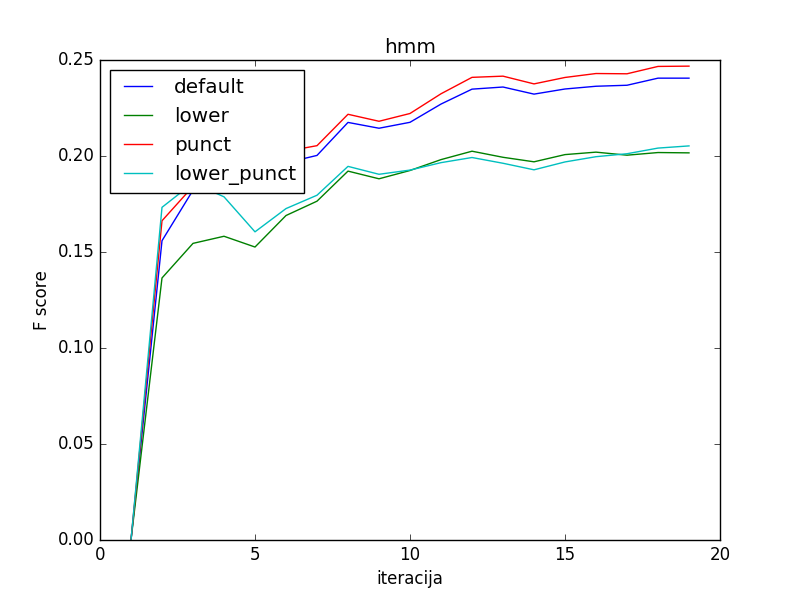
\includegraphics[width=9cm, height=7cm]{hmm.png}
		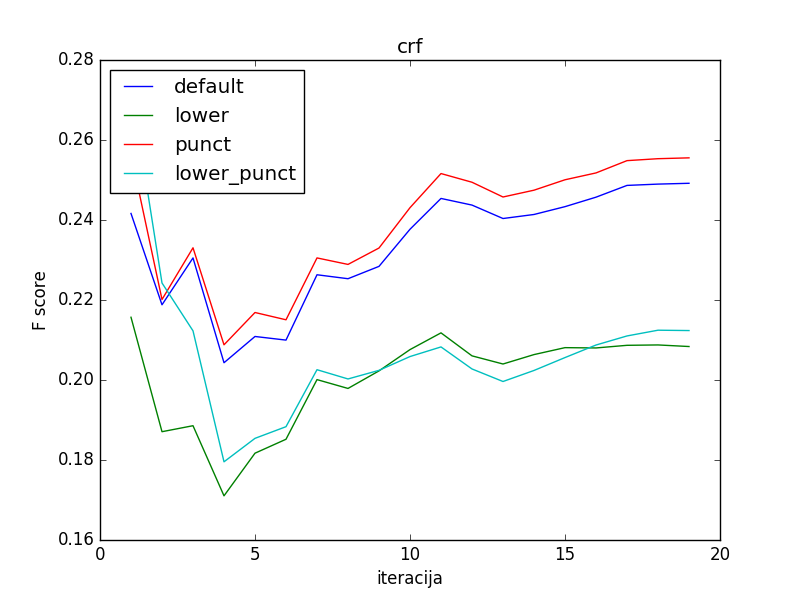
\includegraphics[width=9cm, height=7cm]{crf.png}
		
		Objasnimo značenje svake od naznaka modela:
		\begin{itemize}
			\item Naznaka \textit{default} označava da se u modelu ne koriste interpunkcijski znakovi te da se koristi izvoran oblik riječi (ne pisan malim slovima).
			\item Naznaka \textit{punct} označava da se u modelu koriste interpunkcijski znakovi te da se koristi izvoran oblik riječi
			\item Naznaka \textit{lower} označava da se u modelu koriste isključivo riječi pisane malim slovima te da nema interpunkcijskih znakova. 
			\item Naznaka \textit{lower punct} označava da se u modelu koriste isključivo riječi pisane malim slovima te da se koriste interpunkcijski znakovi.
		\end{itemize}
		
		Kao što vidimo, najuspješniji modeli pri unakrsnoj validaciji su bili oni koji su pri treniranju koristili i riječi i interpunkcijske znakove, te koji nisu koristili tekst pisan samo malim slovima. Modeli koji su koristili riječi pisane malim slovima su postigli znatno lošiji rezultat.
		Također uočavamo i da su CRF i HMM modeli postigli približno jednake rezultate nad skupom za unakrsnu validaciju.
		
	\subsection{Testiranje}
	
		Pri treniranju i unakrsnoj validaciji smo uočili da povećanje skupa za treniranje za samo nekoliko (5-7) priča rezultira primjetno boljim modelima. Stoga je skup priča za testiranje relativno malen te sadrži ukupno sedam nasumično odabranih priča. 
		
		Slijede matrice konfuzije za svaki od modela. 
		 
		Prvi modeli koje smo testirali su četiri HMM modela. Iako su pokazali relativno dobre rezultate nad skupom za unakrsnu validaciju, nad testnim podacima su dali posve negativne rezultate -- niti jednu riječ nisu označili kao lika. Donja tablica daje matricu konfuzije za sve četiri varijante. Naravno, pripadni $F_2$ score je nula.
		
		\vspace{1em}
		\begin{tabular}{|l|l|l|l|}
			\hline
			\multicolumn{2}{|l|}{{\color[HTML]{000000} }}                                                                                                              & \multicolumn{2}{c|}{\cellcolor[HTML]{C0C0C0}{\color[HTML]{000000} \textbf{Oznake modela}}}                                                  \\ \cline{3-4} 
			\multicolumn{2}{|l|}{\multirow{-2}{*}{{\color[HTML]{000000} HMM svi modeli}}}                                                                                 & \cellcolor[HTML]{EFEFEF}{\color[HTML]{000000} \textbf{Likovi}} & \cellcolor[HTML]{EFEFEF}{\color[HTML]{000000} \textbf{Nisu likovi}} \\ \hline
			\multicolumn{1}{|c|}{\cellcolor[HTML]{C0C0C0}}                                       & \cellcolor[HTML]{EFEFEF}{\color[HTML]{000000} \textbf{Likovi}}      & {\color[HTML]{000000} 0}                                       & {\color[HTML]{000000} 86}                                           \\ \cline{2-4} 
			\multicolumn{1}{|c|}{\multirow{-2}{*}{\cellcolor[HTML]{C0C0C0}\textbf{Točne oznake}}} & \cellcolor[HTML]{EFEFEF}{\color[HTML]{000000} \textbf{Nisu likovi}} & {\color[HTML]{000000} 0}                                       & {\color[HTML]{000000} 5366}                                         \\ \hline
		\end{tabular}
		
		\vspace{2em}
		Sljedeći po redu su CRF modeli. Oni su se pokazali prihvatljivima nad testnim skupom, ali nisu dali dovoljno dobre rezultate. Modeli koji u obzir uzima interpunkcije te riječi u izvornom obliku se pokazao najboljim. Najlošiji model ne uzima interpunkcije niti velika slova u obzir.
		
		\vspace{1em}
		\begin{tabular}{|l|l|l|l|}
			\hline
			\multicolumn{2}{|l|}{{\color[HTML]{000000} }}                                                                                                              & \multicolumn{2}{c|}{\cellcolor[HTML]{C0C0C0}{\color[HTML]{000000} \textbf{Oznake modela}}}                                                  \\ \cline{3-4} 
			\multicolumn{2}{|l|}{\multirow{-2}{*}{{\color[HTML]{000000} CRF default}}}                                                                                 & \cellcolor[HTML]{EFEFEF}{\color[HTML]{000000} \textbf{Likovi}} & \cellcolor[HTML]{EFEFEF}{\color[HTML]{000000} \textbf{Nisu likovi}} \\ \hline
			\multicolumn{1}{|c|}{\cellcolor[HTML]{C0C0C0}}                                       & \cellcolor[HTML]{EFEFEF}{\color[HTML]{000000} \textbf{Likovi}}      & {\color[HTML]{000000} 32}                                      & {\color[HTML]{000000} 54}                                           \\ \cline{2-4} 
			\multicolumn{1}{|c|}{\multirow{-2}{*}{\cellcolor[HTML]{C0C0C0}\textbf{Točne oznake}}} & \cellcolor[HTML]{EFEFEF}{\color[HTML]{000000} \textbf{Nisu likovi}} & {\color[HTML]{000000} 52}                                      & {\color[HTML]{000000} 5314}                                         \\ \hline
		\end{tabular}
		
		\begin{align*}
			F_2 = 0.3738
		\end{align*}
		
		\vspace{1em}
		\begin{tabular}{|l|l|l|l|}
			\hline
			\multicolumn{2}{|l|}{{\color[HTML]{000000} }}                                                                                                              & \multicolumn{2}{c|}{\cellcolor[HTML]{C0C0C0}{\color[HTML]{000000} \textbf{Oznake modela}}}                                                  \\ \cline{3-4} 
			\multicolumn{2}{|l|}{\multirow{-2}{*}{{\color[HTML]{000000} CRF punct}}}                                                                                 & \cellcolor[HTML]{EFEFEF}{\color[HTML]{000000} \textbf{Likovi}} & \cellcolor[HTML]{EFEFEF}{\color[HTML]{000000} \textbf{Nisu likovi}} \\ \hline
			\multicolumn{1}{|c|}{\cellcolor[HTML]{C0C0C0}}                                       & \cellcolor[HTML]{EFEFEF}{\color[HTML]{000000} \textbf{Likovi}}      & {\color[HTML]{000000} 33}                                      & {\color[HTML]{000000} 53}                                           \\ \cline{2-4} 
			\multicolumn{1}{|c|}{\multirow{-2}{*}{\cellcolor[HTML]{C0C0C0}\textbf{Točne oznake}}} & \cellcolor[HTML]{EFEFEF}{\color[HTML]{000000} \textbf{Nisu likovi}} & {\color[HTML]{000000} 54}                                      & {\color[HTML]{000000} 5312}                                         \\ \hline
		\end{tabular}
		
		\begin{align*}
			F_2 = 0.3828
		\end{align*}
		
		\vspace{1em}
		\begin{tabular}{|l|l|l|l|}
			\hline
			\multicolumn{2}{|l|}{{\color[HTML]{000000} }}                                                                                                              & \multicolumn{2}{c|}{\cellcolor[HTML]{C0C0C0}{\color[HTML]{000000} \textbf{Oznake modela}}}                                                  \\ \cline{3-4} 
			\multicolumn{2}{|l|}{\multirow{-2}{*}{{\color[HTML]{000000} CRF lower}}}                                                                                 & \cellcolor[HTML]{EFEFEF}{\color[HTML]{000000} \textbf{Likovi}} & \cellcolor[HTML]{EFEFEF}{\color[HTML]{000000} \textbf{Nisu likovi}} \\ \hline
			\multicolumn{1}{|c|}{\cellcolor[HTML]{C0C0C0}}                                       & \cellcolor[HTML]{EFEFEF}{\color[HTML]{000000} \textbf{Likovi}}      & {\color[HTML]{000000} 25}                                      & {\color[HTML]{000000} 61}                                           \\ \cline{2-4} 
			\multicolumn{1}{|c|}{\multirow{-2}{*}{\cellcolor[HTML]{C0C0C0}\textbf{Točne oznake}}} & \cellcolor[HTML]{EFEFEF}{\color[HTML]{000000} \textbf{Nisu likovi}} & {\color[HTML]{000000} 47}                                      & {\color[HTML]{000000} 5319}                                         \\ \hline
		\end{tabular}
		
		\begin{align*}
			F_2 = 0.3005
		\end{align*}
		
		\vspace{1em}
		\begin{tabular}{|l|l|l|l|}
			\hline
			\multicolumn{2}{|l|}{{\color[HTML]{000000} }}                                                                                                              & \multicolumn{2}{c|}{\cellcolor[HTML]{C0C0C0}{\color[HTML]{000000} \textbf{Oznake modela}}}                                                  \\ \cline{3-4} 
			\multicolumn{2}{|l|}{\multirow{-2}{*}{{\color[HTML]{000000} CRF lower punct}}}                                                                                 & \cellcolor[HTML]{EFEFEF}{\color[HTML]{000000} \textbf{Likovi}} & \cellcolor[HTML]{EFEFEF}{\color[HTML]{000000} \textbf{Nisu likovi}} \\ \hline
			\multicolumn{1}{|c|}{\cellcolor[HTML]{C0C0C0}}                                       & \cellcolor[HTML]{EFEFEF}{\color[HTML]{000000} \textbf{Likovi}}      & {\color[HTML]{000000} 27}                                      & {\color[HTML]{000000} 59}                                           \\ \cline{2-4} 
			\multicolumn{1}{|c|}{\multirow{-2}{*}{\cellcolor[HTML]{C0C0C0}\textbf{Točne oznake}}} & \cellcolor[HTML]{EFEFEF}{\color[HTML]{000000} \textbf{Nisu likovi}} & {\color[HTML]{000000} 36}                                      & {\color[HTML]{000000} 5330}                                         \\ \hline
		\end{tabular}
		
		\begin{align*}
			F_2 = 0.3317
		\end{align*}
		
		\vspace{1em}
		Posljednji na redu su Stanford NER modeli. S obzirom da je Stanford NER razvijan godinama od strane vrhunskih stručnjaka i znanstvenika, očekivali smo da će dati najbolje rezultate. Naša očekivanja su se ostvarila, što je vidljivo iz donjih tablica. Najbolji rezultati su ostvareni uz riječi u izvornom obliku i uklanjanje interpunkcijskih znakova iz teksta. Najlošiji rezultati su ostvareni u suprotnom slučaju, uz riječi pisane malim slovima i interpunkcijske znakove.
		
		\vspace{1em}
		\begin{tabular}{|l|l|l|l|}
			\hline
			\multicolumn{2}{|l|}{{\color[HTML]{000000} }}                                                                                                              & \multicolumn{2}{c|}{\cellcolor[HTML]{C0C0C0}{\color[HTML]{000000} \textbf{Oznake modela}}}                                                  \\ \cline{3-4} 
			\multicolumn{2}{|l|}{\multirow{-2}{*}{{\color[HTML]{000000} Stanford NER default }}}                                                                                 & \cellcolor[HTML]{EFEFEF}{\color[HTML]{000000} \textbf{Likovi}} & \cellcolor[HTML]{EFEFEF}{\color[HTML]{000000} \textbf{Nisu likovi}} \\ \hline
			\multicolumn{1}{|c|}{\cellcolor[HTML]{C0C0C0}}                                       & \cellcolor[HTML]{EFEFEF}{\color[HTML]{000000} \textbf{Likovi}}      & {\color[HTML]{000000} 55}                                      & {\color[HTML]{000000} 55}                                           \\ \cline{2-4} 
			\multicolumn{1}{|c|}{\multirow{-2}{*}{\cellcolor[HTML]{C0C0C0}\textbf{Točne oznake}}} & \cellcolor[HTML]{EFEFEF}{\color[HTML]{000000} \textbf{Nisu likovi}} & {\color[HTML]{000000} 31}                                      & {\color[HTML]{000000} 5311}                                         \\ \hline
		\end{tabular}
		
		\begin{align*}
			F_2 = 0.6057
		\end{align*}
		
		\vspace{1em}
		\begin{tabular}{|l|l|l|l|}
			\hline
			\multicolumn{2}{|l|}{{\color[HTML]{000000} }}                                                                                                              & \multicolumn{2}{c|}{\cellcolor[HTML]{C0C0C0}{\color[HTML]{000000} \textbf{Oznake modela}}}                                                  \\ \cline{3-4} 
			\multicolumn{2}{|l|}{\multirow{-2}{*}{{\color[HTML]{000000} NER punct}}}                                                                                 & \cellcolor[HTML]{EFEFEF}{\color[HTML]{000000} \textbf{Likovi}} & \cellcolor[HTML]{EFEFEF}{\color[HTML]{000000} \textbf{Nisu likovi}} \\ \hline
			\multicolumn{1}{|c|}{\cellcolor[HTML]{C0C0C0}}                                       & \cellcolor[HTML]{EFEFEF}{\color[HTML]{000000} \textbf{Likovi}}      & {\color[HTML]{000000} 48}                                      & {\color[HTML]{000000} 38}                                           \\ \cline{2-4} 
			\multicolumn{1}{|c|}{\multirow{-2}{*}{\cellcolor[HTML]{C0C0C0}\textbf{Točne oznake}}} & \cellcolor[HTML]{EFEFEF}{\color[HTML]{000000} \textbf{Nisu likovi}} & {\color[HTML]{000000} 30}                                      & {\color[HTML]{000000} 5326}                                         \\ \hline
		\end{tabular}
		
		\begin{align*}
			F_2 = 0.5556
		\end{align*}
		
		\vspace{1em}
		\begin{tabular}{|l|l|l|l|}
			\hline
			\multicolumn{2}{|l|}{{\color[HTML]{000000} }}                                                                                                              & \multicolumn{2}{c|}{\cellcolor[HTML]{C0C0C0}{\color[HTML]{000000} \textbf{Oznake modela}}}                                                  \\ \cline{3-4} 
			\multicolumn{2}{|l|}{\multirow{-2}{*}{{\color[HTML]{000000} NER lower}}}                                                                                 & \cellcolor[HTML]{EFEFEF}{\color[HTML]{000000} \textbf{Likovi}} & \cellcolor[HTML]{EFEFEF}{\color[HTML]{000000} \textbf{Nisu likovi}} \\ \hline
			\multicolumn{1}{|c|}{\cellcolor[HTML]{C0C0C0}}                                       & \cellcolor[HTML]{EFEFEF}{\color[HTML]{000000} \textbf{Likovi}}      & {\color[HTML]{000000} 41}                                      & {\color[HTML]{000000} 45}                                           \\ \cline{2-4} 
			\multicolumn{1}{|c|}{\multirow{-2}{*}{\cellcolor[HTML]{C0C0C0}\textbf{Točne oznake}}} & \cellcolor[HTML]{EFEFEF}{\color[HTML]{000000} \textbf{Nisu likovi}} & {\color[HTML]{000000} 66}                                      & {\color[HTML]{000000} 5300}                                         \\ \hline
		\end{tabular}
		
		\begin{align*}
			F_2 = 0.4545
		\end{align*}
		
		\vspace{1em}
		\begin{tabular}{|l|l|l|l|}
			\hline
			\multicolumn{2}{|l|}{{\color[HTML]{000000} }}                                                                                                              & \multicolumn{2}{c|}{\cellcolor[HTML]{C0C0C0}{\color[HTML]{000000} \textbf{Oznake modela}}}                                                  \\ \cline{3-4} 
			\multicolumn{2}{|l|}{\multirow{-2}{*}{{\color[HTML]{000000} NER lower punct }}}                                                                                 & \cellcolor[HTML]{EFEFEF}{\color[HTML]{000000} \textbf{Likovi}} & \cellcolor[HTML]{EFEFEF}{\color[HTML]{000000} \textbf{Nisu likovi}} \\ \hline
			\multicolumn{1}{|c|}{\cellcolor[HTML]{C0C0C0}}                                       & \cellcolor[HTML]{EFEFEF}{\color[HTML]{000000} \textbf{Likovi}}      & {\color[HTML]{000000} 30}                                      & {\color[HTML]{000000} 56}                                           \\ \cline{2-4} 
			\multicolumn{1}{|c|}{\multirow{-2}{*}{\cellcolor[HTML]{C0C0C0}\textbf{Točne oznake}}} & \cellcolor[HTML]{EFEFEF}{\color[HTML]{000000} \textbf{Nisu likovi}} & {\color[HTML]{000000} 36}                                      & {\color[HTML]{000000} 5300}                                         \\ \hline
		\end{tabular}
		
		\begin{align*}
			F_2 = 0.3659
		\end{align*}
		
		
\section{Mogući budući nastavak istraživanja}
	
	Tijekom izrade ovog rada susreli smo se s problemom nedostupnosti podataka. Najsličniji i najčešći problem ove vrste u obzir uzima isključivo imenovane entiteta, odnosno imena osoba i nazive lokacija. Za taj problem postoje javno dostupni veliki skupovi označenih podataka, poput novinskih tekstova, ali takvi podaci nama nisu odgovarali. Stoga smo bili primorani ručno označavati podatke, što je relativno spor proces. Pretpostavljamo da su loši rezultati, pogotovo na skrivenim Markovljevim modelima, posljedica malog skupa podataka za učenje. Zato kao prvi korak za nastavak istraživanja preporučujemo povećanje skupa na treniranje na barem stotinu priča. Time bismo mogli povećati i veličinu skupa za testiranje, te dobiti vjerodostojnije podatke.
	
	Kao sljedeći korak preporučujemo primjenu ansambla poput \textit{bagginga}, odnosno \textit{boostinga}, u ovisnosti o pristranosti, odnosno eventualnoj varijanci.
	
	Kao posljednji korak spominjemo moguću upotrebu neuralnih mreža. Konvolucijske neuralne mreže su dobar odabir za probleme u analizi teksta, s obzirom da pri učenju u obzir uzimaju okolinu (kontekst) svake riječi. Ipak, dosadašnja istraživanja pokazuju kako su metode poput skrivenih Markovljevih modela i uvjetnih nasumičnih polja jednako dobar ili bolji izbor. Također, veliki nedostatak neuralnih mreža je taj da zahtijevaju velik skup podataka za učenje. S obzirom da smo već naveli da je podatke potrebno ručno označavati, to bi moglo predstavljati veliki problem.

\section{Zaključak}
		
	Problem prepoznavanja imenovanih entiteta (NER) u tekstu se proučava već duže vrijeme, od sedamdesetih godina prošlog stoljeća. Primarno je cilj bio otkriti koje riječi predstavljaju ime osobe, naziv lokacije ili naziv organizacije u tekstu, najčešće novinskim člancima. Danas uspješna rješenja ovog problema donose financijsku korist. Naime, pretežno se koriste u oglašavanju, na primjer uz ime lokacije u članku nekog web portala možemo vezati oglas za hotel. Druga primjena je u označavanju i istraživanju biljnih, ljudskih i životinjskih gena i genoma.
	
	Naš pristup je jako rijedak, pa ne postoje javno dostupni podaci za učenje u obliku anotiranih priča. Unatoč tome, uspjeli smo istrenirati relativno dobar model za prepoznavanje likova koristeći Stanford NER, izuzetno uspješan i godinama razvijan NER sustav. Očekujemo da bismo dobili bolje rezultate uz veći skup podataka za učenje.


\begin{thebibliography}{1}
\bibitem{1}
M.~Rudman, \emph{Kompleksnost skrivenih Markovljevih modela}, (diplomski rad).\hskip 1em plus
  0.5em minus 0.4em\relax Prirodoslovno-matematički fakultet, 2014.
  
\bibitem{2}
I.~Medic, \emph{Uslovna slučajna polja}, (master rad).\hskip 1em plus
  0.5em minus 0.4em\relax  Univerzitet u Beogradu, Matematički fakultet, 2013
  
\bibitem{3}
\textit{Stanford Named Entity Recognizer}, The Stanford Natural Language Processing Group, \url{http://nlp.stanford.edu/software/CRF-NER.shtml}

\end{thebibliography}  


\end{document}


